        %%******************************************%%
        %%                                          %%
        %%        Modello di tesi di laurea         %%
        %%            di Andrea Giraldin            %%
        %%                                          %%
        %%             2 novembre 2012              %%
        %%                                          %%
        %%******************************************%%


% I seguenti commenti speciali impostano:
% 1. 
% 2. PDFLaTeX come motore di composizione;
% 3. tesi.tex come documento principale;
% 4. il controllo ortografico italiano per l'editor.

% !TEX encoding = UTF-8
% !TEX TS-program = pdflatex
% !TEX root = tesi.tex
% !TEX spellcheck = it-IT

\documentclass[10pt,                    % corpo del font principale
               a4paper,                 % carta A4
               twoside,                 % impagina per fronte-retro
               openright,               % inizio capitoli a destra
               english,                 
               italian,
               openany,
               ]{book}    

%**************************************************************
% Importazione package
%************************************************************** 

%\usepackage{amsmath,amssymb,amsthm}    % matematica

\usepackage[T1]{fontenc}                % codifica dei font:
                                        % NOTA BENE! richiede una distribuzione *completa* di LaTeX

\usepackage[utf8]{inputenc}             % codifica di input; anche [latin1] va bene
                                        % NOTA BENE! va accordata con le preferenze dell'editor

\usepackage[english, italian]{babel}    % per scrivere in italiano e in inglese;
                                        % l'ultima lingua (l'italiano) risulta predefinita

\usepackage{bookmark}                   % segnalibri

\usepackage{caption}                    % didascalie

\usepackage{chngpage,calc}              % centra il frontespizio

\usepackage{csquotes}                   % gestisce automaticamente i caratteri (")

\usepackage{emptypage}                  % pagine vuote senza testatina e piede di pagina

\usepackage{epigraph}			% per epigrafi

\usepackage{eurosym}                    % simbolo dell'euro

%\usepackage{indentfirst}               % rientra il primo paragrafo di ogni sezione

\usepackage{graphicx}                   % immagini

\usepackage{hyperref}        % collegamenti ipertestuali

\usepackage[binding=5mm]{layaureo}      % margini ottimizzati per l'A4; rilegatura di 5 mm

\usepackage{listings}                   % codici

\usepackage{microtype}                  % microtipografia

\usepackage{mparhack,relsize}  % finezze tipografiche

\usepackage{nameref}                    % visualizza nome dei riferimenti                                      

\usepackage[font=small]{quoting}        % citazioni

\usepackage{subfig}                     % sottofigure, sottotabelle

\usepackage[italian]{varioref}          % riferimenti completi della pagina

\usepackage[dvipsnames]{xcolor}        % colori

\usepackage{booktabs}                   % tabelle                                       
\usepackage{tabularx}                   % tabelle di larghezza prefissata                                    
\usepackage{longtable}                  % tabelle su più pagine                                        
\usepackage{ltxtable}                   % tabelle su più pagine e adattabili in larghezza

\usepackage[toc, acronym]{glossaries}   % glossario
                                        % per includerlo nel documento bisogna:
                                        % 1. compilare una prima volta tesi.tex;
                                        % 2. eseguire: makeindex -s tesi.ist -t tesi.glg -o tesi.gls tesi.glo
                                        % 3. eseguire: makeindex -s tesi.ist -t tesi.alg -o tesi.acr tesi.acn
                                        % 4. compilare due volte tesi.tex.

\usepackage[backend=biber,style=verbose-ibid,hyperref,backref]{biblatex}
                                        % eccellente pacchetto per la bibliografia; 
                                        % produce uno stile di citazione autore-anno; 
                                        % lo stile "numeric-comp" produce riferimenti numerici
                                        % per includerlo nel documento bisogna:
                                        % 1. compilare una prima volta tesi.tex;
                                        % 2. eseguire: biber tesi
                                        % 3. compilare ancora tesi.tex.

\usepackage{titlesec}
\titlespacing*{\section}{0pt}{1.1\baselineskip}{\baselineskip}

\titlespacing*{\subsection}{0pt}{1.1\baselineskip}{\baselineskip}

%**************************************************************
% file contenente le impostazioni della tesi
%**************************************************************

%**************************************************************
% Frontespizio
%**************************************************************

% Autore
\newcommand{\myName}{Francesco De Filippis}                                    
\newcommand{\myTitle}{Autenticazione per Zimbra Collaboration Suite (ZCS) tramite protocollo SAML}

% Tipo di tesi                   
\newcommand{\myDegree}{Tesi di laurea triennale}

% Università             
\newcommand{\myUni}{Università degli Studi di Padova}

% Facoltà       
\newcommand{\myFaculty}{Corso di Laurea in Informatica}

% Dipartimento
\newcommand{\myDepartment}{Dipartimento di Matematica "Tullio Levi-Civita"}

% Titolo del relatore
\newcommand{\profTitle}{Prof.}

% Relatore
\newcommand{\myProf}{Tullio Vardanega}

% Luogo
\newcommand{\myLocation}{Padova}

% Anno accademico
\newcommand{\myAA}{2019-2020}

% Data discussione
\newcommand{\myTime}{26-02-2020}


%**************************************************************
% Impostazioni di impaginazione
% see: http://wwwcdf.pd.infn.it/AppuntiLinux/a2547.htm
%**************************************************************

\setlength{\parindent}{14pt}   % larghezza rientro della prima riga
\setlength{\parskip}{0pt}   % distanza tra i paragrafi


%**************************************************************
% Impostazioni di biblatex
%**************************************************************
\bibliography{bibliografia} % database di biblatex 

\defbibheading{bibliography} {
    \cleardoublepage
    \phantomsection 
    \addcontentsline{toc}{chapter}{\bibname}
    \chapter*{\bibname\markboth{\bibname}{\bibname}}
}

\setlength\bibitemsep{1.5\itemsep} % spazio tra entry

\DeclareBibliographyCategory{opere}
\DeclareBibliographyCategory{web}

\addtocategory{opere}{womak:lean-thinking}
\addtocategory{web}{site:agile-manifesto}

\defbibheading{opere}{\section*{Riferimenti bibliografici}}
\defbibheading{web}{\section*{Siti Web consultati}}


%**************************************************************
% Impostazioni di caption
%**************************************************************
\captionsetup{
    tableposition=top,
    figureposition=bottom,
    font=small,
    format=hang,
    labelfont=bf
}

%**************************************************************
% Impostazioni di glossaries
%**************************************************************
%**************************************************************
% Glossario
%**************************************************************
%\renewcommand{\glossaryname}{Glossario}

\newglossaryentry{zcsg}
{
    name=\glslink{zcs}{ZCS},
    text=Zimbra,
    sort=zimbra,
    description={Zimbra \textit{Collaboration}}
}

\newglossaryentry{spg}
{
    name=\glslink{sp}{SP},
    text=SP,
    sort=service provider,
    description={Un \textit{service provider} è un sistema che fornisce un servizio a degli utenti. Lo si può identificare come un sito web che eroga un certo servizio}
}

\newglossaryentry{idpg}
{
    name=\glslink{idp}{IdP},
    text=IdP,
    sort=identity provider,
    description={Un \textit{identity provider} è un sistema che crea, mantiene e gestisce le informazioni sull'identità di un utente. Si occupa di fornire il servizio di autenticazione ai \gls{spg}}
}

\newglossaryentry{okta}
{
    name=\glslink{okta}{Okta},
    text=Okta,
    sort=okta,
    description={Okta è una società di gestione di identità e di accessi, quindi un \gls{idpg}}
}

\newglossaryentry{xmlg}
{
    name=\glslink{xml}{XML},
    text=XML,
    sort=xml,
    description={Linguaggio di \textit{\textbf{Markup}} che consente la definizione di \textbf{metadati}}
}

\newglossaryentry{samlg}
{
    name=\glslink{saml}{SAML},
    text=SAML,
    sort=saml,
    description={SAML è un protocollo bastato su \gls{xmlg} che permette lo scambio di messaggi per effettuare autenticazione e autorizzazione tra domini distinti. Tipicamente gli attori del procollo sono un \gls{idpg} che fornisce l'identità dell'utente da autenticare e un \gls{spg} che fornisce il servizio a cui l'utente ha richiesto l'accesso. }
}

\newglossaryentry{ssog}
{
    name=\glslink{sso}{SSO},
    text=Single Sign-On,
    sort=sso,
    description={Si tratta di un sistema di autenticazione che permette ad un utente di effettuare un'unica autenticazione, valida per più servizi e/o risorse ai quali è abilitato. Questo permette all'utente di avere un'unica credenziale valida per più servizi indipendenti}
}

\newglossaryentry{samlass}
{
    name=\glslink{samlass}{SAML Assertion},
    text=SAML Assertion,
    sort=saml assertion,
    description={Una asserzione \gls{samlg} è un documento in formato \gls{xmlg} che contiene le informazioni sull'autenticazione e/o autorizzazione di un utente. Tale documento è solitamente generato dall'\gls{idpg} e inviato al \gls{spg}}
}

\newglossaryentry{crudg}
{
    name=\glslink{crud}{CRUD},
    text=CRUD,
    sort=crud,
    description={Questo acronimo viene spesso usato in ambito di \textbf{database management} e indica:
    \begin{itemize}
        \item \textbf{Create}: creazione di un utente;
        \item \textbf{Read}: richiesta attributi di un utente;
        \item \textbf{Update}: aggiornamento attributi di un utente;
        \item \textbf{Delete}: non si parla di una cancellazione vera e propria di un utente ma di \textbf{deprovisioning}, ovvero una disabilitazione dell'\textit{account} di quest'ultimo o di un cambio di permessi
    \end{itemize}}
}

\newglossaryentry{prov}
{
    name=\glslink{prov}{Provisioning},
    text=Provisioning,
    sort=provisioning,
    description={Con il termine \textit{\textbf{provisioning}} si intende, generalmente, la gestione degli utenti. Questo termine include un insieme di funzionalità riassunte dall'acronimo \gls{crudg}}
}

\newglossaryentry{opensg}
{
    name=\glslink{opensg}{Open Source},
    text=open source,
    sort=open source,
    description={Con il termine \textit{\textbf{open source}} si fa riferimento ad un \textit{software} la cui lincenza permette di utilizzarlo, modificarlo e redistribuirlo}
}

\newglossaryentry{closedg}
{
    name=\glslink{closedg}{Closed Source},
    text=closed source,
    sort=closed source,
    description={Con il termine \textit{\textbf{closed source}} si fa riferimento ad un software proprietario, quindi non disponibile pubblicamente}
}

\newglossaryentry{pluging}
{
    name=\glslink{pluging}{Plug-in},
    text=plug-in,
    sort=plugin,
    description={Componente \textit{software} che aggiunge funzionalità all'applicazione su cui viene installato}
}

\newglossaryentry{backupg}
{
    name=\glslink{backupg}{Backup},
    text=backup,
    sort=backup,
    description={Quando si parla di \textit{backup}, si fa riferimento al processo di duplicazione di dati su più supporti (fisici o cloud) al fine di poterli recuperare in caso di perdita inattesa}
}

\newglossaryentry{realtimeg}
{
    name=\glslink{realtimeg}{Real-time},
    text=real-time,
    sort=realtime,
    description={\textit{Software} che opera sotto condizioni temporali ben definite}
}

\newglossaryentry{userexpg}
{
    name=\glslink{userexpg}{User experience},
    text=user experience,
    sort=user experience,
    description={L'esperienza che manifesta l'utente, nell'interagire con un certo prodotto, sistema o servizio}
}

\newglossaryentry{agileg}
{
    name=\glslink{agileg}{Agile},
    text=agile,
    sort=agile,
    description={Approccio allo sviluppo software che pone il focus sul consegnare al cliente un \textit{software} completo, funzionante  e di qualità in tempi brevi}
}

\newglossaryentry{frameworkg}
{
    name=\glslink{frameworkg}{Framework},
    text=framework,
    sort=framework,
    description={Insieme di strumenti che definiscono la struttura di un sistema a livello concettuale. Nel caso del software si può intedendere come un'architettura sulla quale basare lo sviluppo di un prodotto. Quando si parla di modello di sviluppo si intende l'insieme di strumenti teorici che permettono di mettere in atto un concetto specifico}
}

\newglossaryentry{taskg}
{
    name=\glslink{taskg}{Task},
    text=task,
    sort=task,
    description={Incarico di piccole dimensione assegnato ad un soggetto che dovrà portarlo a termine}
}

\newglossaryentry{wysiwygg}
{
    name=\glslink{wysiwygg}{WYSIWYG},
    text=WYSIWYG,
    sort=wysiwyg,
    description={Sta per "\textit{What You See Is What You Get}" e si riferisce ad una tipologia di \textit{editor} di testo in grado di mostrare in tempo reale, durante la scrittura, quale sarà l'aspetto finale del documento}
}

\newglossaryentry{repositoryg}
{
    name=\glslink{repositoryg}{Repository},
    text=repository,
    sort=repository,
    description={Nell'ambito dello sviluppo software rappresenta un contenitore di codice sorgente, gestito da un sistema di versionamento}
}

\newglossaryentry{workflowg}
{
    name=\glslink{workflowg}{Workflow},
    text=workflow,
    sort=workflowg,
    description={Flusso di esecuzione di un insieme di attività}
}

\newglossaryentry{codereviewg}
{
    name=\glslink{codereviewg}{Code Review},
    text=code review,
    sort=code review,
    description={Attività di revisione del codice effttuata da persone diverse dagli autori, al fine di correggere errori, migliorarne la qualità ed eventualmente proporre soluzioni alternative}
}

\newglossaryentry{itsg}
{
    name=\glslink{itsg}{Issue Tracing System},
    text=issue tracking system,
    sort=issue tracking system,
    description={Software che permette di gestire in maniera ordinata un insieme di issue, ovvero dei \textit{\gls{taskg}} da svolgere. Tipicamente viene utilizzato in ambito collaborativo in quanto permette di tenere traccia delle \textit{issue} risolte da tutti i membri del \textit{team}}
}

\newglossaryentry{cig}
{
    name=\glslink{cig}{Continuous Integration},
    text=continuous integration,
    sort=continuous integration,
    description={Pratica nell'ambito dell'ingeneria del software che consiste nel effettuare \textit{merge} frequenti nella \textit{codebase}, al fine di aggiungere in modo graduale le nuove modifiche, assicurando l'assenza di conflitti tra le nuove modifiche e quelle precedenti}
}

\newglossaryentry{cdg}
{
    name=\glslink{cdg}{Continuous Delivery},
    text=continuous delivery,
    sort=continuous delivery,
    description={Pratica nell'ambito dell'ingeneria del software che consiste nel rilasciare la build di un software pronta per l'ambiente di produzione}
}

\newglossaryentry{bugg}
{
    name=\glslink{bugg}{Bug},
    text=bug,
    sort=bug ,
    description={In informatica si tratta di un errore nel software che produce risultati inattesi}
}

\newglossaryentry{cloudg}
{
    name=\glslink{cloudg}{Cloud},
    text=cloud,
    sort=cloud,
    description={In informatica si tratta di un errore nel software che produce risultati inattesi}
}


%**************************************************************
% Acronimi
%**************************************************************
\renewcommand{\acronymname}{Acronimi e abbreviazioni}

\newacronym[description={\glslink{zcsg}{Zimbra Collaboration Suite}}]
    {zcs}{ZCS}{Zimbra Collaboration Suite}
    
\newacronym[description={\glslink{idpg}{Identity Provider}}]
    {idp}{IdP}{Identity Provider}

\newacronym[description={\glslink{spg}{Identity Provider}}]
    {sp}{SP}{Service Provider}
    
\newacronym[description={\glslink{samlg}{Security Assertion Markup Language}}]
    {saml}{SAML}{Security Assertion Markup Language}
    
\newacronym[description={\glslink{xmlg}{eXtensible Markup Language}}]
    {xml}{XML}{eXtensible Markup Language}
    
\newacronym[description={\glslink{ssog}{Single Sign-On}}]
    {sso}{SSO}{Single Sign-On}
    
\newacronym[description={\glslink{crudg}{Create-Read-Update-Delete}}]
    {crud}{CRUD}{Create-Read-Update-Delete} % database di termini
\makeglossaries


%**************************************************************
% Impostazioni di graphicx
%**************************************************************
\graphicspath{{immagini/}} % cartella dove sono riposte le immagini


%**************************************************************
% Impostazioni di hyperref
%**************************************************************
\hypersetup{
    %hyperfootnotes=false,
    %pdfpagelabels,
    %draft,	% = elimina tutti i link (utile per stampe in bianco e nero)
    colorlinks=true,
    linktocpage=true,
    pdfstartpage=1,
    pdfstartview=FitV,
    % decommenta la riga seguente per avere link in nero (per esempio per la stampa in bianco e nero)
    %colorlinks=false, linktocpage=false, pdfborder={0 0 0}, pdfstartpage=1, pdfstartview=FitV,
    breaklinks=true,
    pdfpagemode=UseNone,
    pageanchor=true,
    pdfpagemode=UseOutlines,
    plainpages=false,
    bookmarksnumbered,
    bookmarksopen=true,
    bookmarksopenlevel=1,
    hypertexnames=true,
    pdfhighlight=/O,
    %nesting=true,
    %frenchlinks,
    urlcolor=webbrown,
    linkcolor=RoyalBlue,
    citecolor=webgreen,
    %pagecolor=RoyalBlue,
    %urlcolor=Black, linkcolor=Black, citecolor=Black, %pagecolor=Black,
    pdftitle={\myTitle},
    pdfauthor={\textcopyright\ \myName, \myUni, \myFaculty},
    pdfsubject={},
    pdfkeywords={},
    pdfcreator={pdfLaTeX},
    pdfproducer={LaTeX}
}

%**************************************************************
% Impostazioni di itemize
%**************************************************************
%\renewcommand{\labelitemi}{$\ast$}

%\renewcommand{\labelitemi}{$\bullet$}
%\renewcommand{\labelitemii}{$\cdot$}
%\renewcommand{\labelitemiii}{$\diamond$}
%\renewcommand{\labelitemiv}{$\ast$}


%**************************************************************
% Impostazioni di listings
%**************************************************************
\lstset{
    language=[LaTeX]Tex,%C++,
    keywordstyle=\color{RoyalBlue}, %\bfseries,
    basicstyle=\small\ttfamily,
    %identifierstyle=\color{NavyBlue},
    commentstyle=\color{Green}\ttfamily,
    stringstyle=\rmfamily,
    numbers=none, %left,%
    numberstyle=\scriptsize, %\tiny
    stepnumber=5,
    numbersep=8pt,
    showstringspaces=false,
    breaklines=true,
    frameround=ftff,
    frame=single
} 


%**************************************************************
% Impostazioni di xcolor
%**************************************************************
\definecolor{webgreen}{rgb}{0,.5,0}
\definecolor{webbrown}{rgb}{.6,0,0}


%**************************************************************
% Altro
%**************************************************************

\newcommand{\omissis}{[\dots\negthinspace]} % produce [...]

% eccezioni all'algoritmo di sillabazione
\hyphenation
{
    ma-cro-istru-zio-ne
    gi-ral-din
}

\newcommand{\sectionname}{sezione}
\addto\captionsitalian{\renewcommand{\figurename}{Figura}
                       \renewcommand{\tablename}{Tabella}}

\newcommand{\glsfirstoccur}{\ap{{[g]}}}

\newcommand{\intro}[1]{\emph{\textsf{#1}}}

%**************************************************************
% Environment per ``rischi''
%**************************************************************
\newcounter{riskcounter}                % define a counter
\setcounter{riskcounter}{0}             % set the counter to some initial value

%%%% Parameters
% #1: Title
\newenvironment{risk}[1]{
    \refstepcounter{riskcounter}        % increment counter
    \par \noindent                      % start new paragraph
    \textbf{\arabic{riskcounter}. #1}   % display the title before the 
                                        % content of the environment is displayed 
}{
    \par\medskip
}

\newcommand{\riskname}{Rischio}

\newcommand{\riskdescription}[1]{\textbf{\\Descrizione:} #1.}

\newcommand{\risksolution}[1]{\textbf{\\Soluzione:} #1.}

%**************************************************************
% Environment per ``use case''
%**************************************************************
\newcounter{usecasecounter}             % define a counter
\setcounter{usecasecounter}{0}          % set the counter to some initial value

%%%% Parameters
% #1: ID
% #2: Nome
\newenvironment{usecase}[2]{
    \renewcommand{\theusecasecounter}{\usecasename #1}  % this is where the display of 
                                                        % the counter is overwritten/modified
    \refstepcounter{usecasecounter}             % increment counter
    \vspace{10pt}
    \par \noindent                              % start new paragraph
    {\large \textbf{\usecasename #1: #2}}       % display the title before the 
                                                % content of the environment is displayed 
    \medskip
}{
    \medskip
}

\newcommand{\usecasename}{UC}

\newcommand{\usecaseactors}[1]{\textbf{\\Attori Principali:} #1. \vspace{4pt}}
\newcommand{\usecasepre}[1]{\textbf{\\Precondizioni:} #1. \vspace{4pt}}
\newcommand{\usecasedesc}[1]{\textbf{\\Descrizione:} #1. \vspace{4pt}}
\newcommand{\usecasepost}[1]{\textbf{\\Postcondizioni:} #1. \vspace{4pt}}
\newcommand{\usecasealt}[1]{\textbf{\\Scenario Alternativo:} #1. \vspace{4pt}}

%**************************************************************
% Environment per ``namespace description''
%**************************************************************

\newenvironment{namespacedesc}{
    \vspace{10pt}
    \par \noindent                              % start new paragraph
    \begin{description} 
}{
    \end{description}
    \medskip
}

\newcommand{\classdesc}[2]{\item[\textbf{#1:}] #2}

%Fonte immagini
\newcommand*{\captionsource}[2]{%
  \caption[{#1}]{%
    #1%
    \\\hspace{\linewidth}%
    \textbf{Fonte:} #2%
  }%
}                     % file con le impostazioni personali

%\usepackage[hidelinks]{hyperref}    %clickable ToC
%\hypersetup{allcolors=black,linktocpage,linktoc=all}

\begin{document}
%**************************************************************
% Materiale iniziale
%**************************************************************
\frontmatter
% !TEX encoding = UTF-8
% !TEX TS-program = pdflatex
% !TEX root = ../tesi.tex

%**************************************************************
% Frontespizio 
%**************************************************************
\begin{titlepage}

\begin{center}

\begin{LARGE}
\textbf{\myUni}\\
\end{LARGE}

\vspace{10pt}

\begin{Large}
\textsc{\myDepartment}\\
\end{Large}

\vspace{10pt}

\begin{large}
\textsc{\myFaculty}\\
\end{large}

\vspace{30pt}
\begin{figure}[htbp]
\begin{center}

\includegraphics[height=6cm]{logo-unipd}
\end{center}
\end{figure}
\vspace{30pt} 

\begin{LARGE}
\begin{center}
\textbf{\myTitle}\\
\end{center}
\end{LARGE}

\vspace{10pt} 

\begin{large}
\textsl{\myDegree}\\
\end{large}

\vspace{40pt} 

\begin{large}
\begin{flushleft}
\textit{Relatore}\\ 
\vspace{5pt} 
\profTitle \myProf
\end{flushleft}

\vspace{0pt} 

\begin{flushright}
\textit{Laureando}\\ 
\vspace{5pt} 
\myName
\end{flushright}
\end{large}

\vspace{40pt}

\line(1, 0){338} \\
\begin{normalsize}
\textsc{Anno Accademico \myAA}
\end{normalsize}

\end{center}
\end{titlepage} 
% !TEX encoding = UTF-8
% !TEX TS-program = pdflatex
% !TEX root = ../tesi.tex

%**************************************************************
% Colophon
%**************************************************************
\clearpage
\phantomsection
\thispagestyle{empty}

\hfill

\vfill

\noindent\myName: \textit{\myTitle,}
\myDegree,
\textcopyright\ \myTime.
% !TEX encoding = UTF-8
% !TEX TS-program = pdflatex
% !TEX root = ../tesi.tex

%**************************************************************
% Ringraziamenti
%**************************************************************
\cleardoublepage
\phantomsection
\pdfbookmark{Ringraziamenti}{ringraziamenti}

\bigskip

\begingroup
\let\clearpage\relax
\let\cleardoublepage\relax
\let\cleardoublepage\relax

\chapter*{Ringraziamenti}

\noindent \textit{Innanzitutto, vorrei esprimere la mia gratitudine al Prof. Tullio Vardanega, relatore della mia tesi, per l'aiuto e il sostegno fornitomi durante la stesura del lavoro.}\\

\noindent \textit{Ringrazio Zextras per l'opportunità e per la professionalità dimostrata. Ringrazio il team The Lucky Gunslingers per avermi guidato durante tutto il corso del progetto.}\\

\noindent \textit{Desidero ringraziare con affetto la mia famiglia per il sostegno, il grande aiuto e per essermi stata vicina in ogni momento durante gli anni di studio.}\\

\noindent \textit{Ringrazio infine i miei amici per le esperienze vissute durante questi anni. In particolar modo Andrea, Michele e Riccardo. Ringrazio inoltre le persone con cui ho avuto modo di condividere il percorso universitario.}\\


\bigskip

\noindent\textit{\myLocation, Febbraio 2020}
\hfill \myName

\endgroup


% !TEX encoding = UTF-8
% !TEX TS-program = pdflatex
% !TEX root = ../tesi.tex

%**************************************************************
% Sommario
%**************************************************************
\cleardoublepage
\phantomsection
\pdfbookmark{Sommario}{Sommario}
\begingroup
\let\clearpage\relax
\let\cleardoublepage\relax
\let\cleardoublepage\relax

\chapter*{Sommario}

Il presente documento descrive il lavoro svolto durante il periodo di stage, della durata di 304 ore, dal laureando Francesco De Filippis presso l'azienda Zextras S.r.l di Torri di Quartesolo (VI).
Gli obiettivi da raggiungere erano molteplici.\\
La prima funzionalità richiesta dall'azienda era l'autenticazione di un utente presente su \gls{zcs} attraverso l'\gls{idp} \gls{okta}, il quale supporta il protocollo \gls{saml}.
Oltre all'autenticazione per gli utenti già esistenti su \gls{zcsg} era richiesto anche il \gls{prov}. In particolare si trattava di creare un nuovo account su \gls{zcsg} al primo tentativo di login dell'utente con conseguente autenticazione. I dati per la creazione dell'utente venivano forniti da \gls{okta} attraverso una \gls{samlass}. Utilizzando questi dati era richiesta la configurazione dell'account creato.\\
Il documento è così suddiviso:
\begin{itemize}
    \item \hyperref[cap:azienda]{Il primo capitolo} descrive l'azienda presso cui ho svolto lo stage. In particolare viene illustrata la sua storia, i suoi prodotti e il modo in cui opera;
    \item \hyperref[cap:obiettivi]{Il secondo capitolo} descrive gli obiettivi dello stage
    in relazione alle aspettative aziendali e personali;
    \item \hyperref[cap:resoconto]{Il terzo capitolo} descrive la scelte progettuali che ho compiuto al fine di proporre una soluzione per soddisfare gli obiettivi prefissati dallo stage;
    \item \hyperref[cap:retrospettiva]{Il quarto capitolo} presenta una valutazione dello stage in relazione agli obiettivi dell'azienda e all'esperienza da me acquisita nel corso del suo svolgimento.
\end{itemize}

%\vfill
%
%\selectlanguage{english}
%\pdfbookmark{Abstract}{Abstract}
%\chapter*{Abstract}
%
%\selectlanguage{italian}

\endgroup			

\vfill


% !TEX encoding = UTF-8
% !TEX TS-program = pdflatex
% !TEX root = ../tesi.tex

%**************************************************************
% Indici
%**************************************************************

\cleardoublepage
\pdfbookmark{\contentsname}{tableofcontents}
\setcounter{tocdepth}{2}
\tableofcontents
%\markboth{\contentsname}{\contentsname} 
\clearpage

\begingroup 
    \let\clearpage\relax
    \let\cleardoublepage\relax
    \let\cleardoublepage\relax
    %*******************************************************
    % Elenco delle figure
    %*******************************************************    
    \phantomsection
    \pdfbookmark{\listfigurename}{lof}
    \listoffigures

    \vspace*{8ex}

    %*******************************************************
    % Elenco delle tabelle
    %*******************************************************
    \phantomsection
    \pdfbookmark{\listtablename}{lot}
    \listoftables
        
    \vspace*{8ex}
\endgroup

\cleardoublepage

\cleardoublepage

%**************************************************************
% Materiale principale
%**************************************************************
\mainmatter
% !TEX encoding = UTF-8
% !TEX TS-program = pdflatex
% !TEX root = ../tesi.tex

%**************************************************************
\chapter{L'azienda}
\label{cap:azienda}
%**************************************************************

%**************************************************************
\section{Profilo aziendale}
    \textbf{Zextras s.r.l.} nasce a Torri di Quartesolo (VI) nel 2011 come estensione di \textbf{Studio Storti s.r.l.} che opera, dal 1997, nel campo delle soluzioni \textit{\gls{opensg}}. Sin dall'inizio, l'obiettivo principale di questa società era quello di estendere \gls{zcsg} \textit{Open Source Edition}, uno dei più diffusi strumenti collaborativi per aziende e pubbliche amministrazioni, aggiungendo nuove funzionalità. \\
    Nel corso degli anni è nata e cresciuta \textbf{Zextras Suite}, una raccolta di estensioni che permettono di arricchire \gls{zcsg} con nuove funzionalità utili nel suo utilizzo in ambito professionale.
    Le soluzioni proposte da \textbf{Zextras} con i sui prodotti vengono da subito apprezzate da \textbf{Synacor}, l'azienda che sviluppa e mantiene \gls{zcsg}, la quale decide di includere parte del suo codice nella versione \textit{\gls{opensg}}. Attualmente i prodotti sviluppati dall'azienda vengono utilizzati da più di 100 milioni di utenti in tutto il mondo.

    \begin{figure}[ht]
            \centering
            
\includegraphics[width=0.8\textwidth]{immagini/opensource.jpeg}
            \caption{\textit{Open source}}
            \textbf{Fonte}: \href{https://miro.medium.com/max/2048/1*MnJBb5qalimr1Ji7bKJctQ.jpeg}{medium.com}
            \label{fig: Open source}
        \end{figure}

\section{Dominio applicativo}
    \subsection{Zimbra Open Source Edition}
        \textbf{Zextras}, come già accennato, è nata con l'obiettivo di creare nuovi contenuti per \gls{zcsg} facendone quindi il suo \textit{core business}.
        \gls{zcsg} è un \textit{software} collaborativo di gruppo adatto a coordinare e supportare l'attività lavorativa di aziende, pubbliche amministrazioni e altri enti. I principali servizi offerti da questo \textit{software} sono i seguenti:
        \begin{itemize}
            \item posta elettronica;
            \item gestione di calendari condivisi e organizzazione eventi;
            \item interfaccia amministratore;
            \item supporto dei servizi su dispositivi mobili.
        \end{itemize}
        Per estendere l'applicativo con ulteriori funzionalità, sviluppate anche da terze parti, è possibile installare un \textit{\gls{pluging}} che in ambiente \gls{zcsg} viene chiamato \textbf{Zimlet}. \\
        Esistono due versioni di \gls{zcsg}:
        \begin{itemize}
            \setlength\itemsep{0em}
            \item \textbf{Zimbra Open Source Edition}: è la versione su cui lavora \textbf{Zextras} e offre i servizi elecanti in precedenza;
            \item \textbf{Zimbra Network Edition}: è una versione a pagamento che offre alcune funzionalità \textit{\gls{closedg}}, tra cui un protocollo per la sincronizzazione di calendario e contatti e maggiori funzionalità per gli amministratori.
        \end{itemize}
        
    \subsection{Zextras Suite}
        \textbf{Zextras Suite} è un insieme di strumenti che permettono di aggiungere delle funzionalità a \gls{zcsg} \textit{Open Source Edition} in modo indipendente da quest'ultimo. Ciò permette una configurazione altamente modulare e personalizzabile in base alle necessità dell'utilizzatore. \\
        Questa \textit{suite} offre i seguenti prodotti:
        \begin{itemize}
            \setlength\itemsep{0em}
            \item \textit{\textbf{Powerstore}}: sistema di ottimizzazione dei dati che permette il risparmio di memoria sui server \gls{zcsg};
            \item \textit{\textbf{Backup}}: motore di \textit{\gls{backupg}} in \textit{\gls{realtimeg}};
            \item \textit{\textbf{Admin}}: strumenti dedicati agli amministratori per la gestione e il monitoraggio dei servizi attivi sull'istanza di \gls{zcsg};
            \item \textit{\textbf{Mobile}}: gestione e sincronizzazione di posta elettronica, contatti, eventi e calendario su dispositivi mobili tramite protocolli \textit{Exchange} e \textit{EAS 16.0 (ActiveSync)};
            \item \textit{\textbf{Chat}}: piattaforma di messaggistica istantanea nativamente integrata in \gls{zcsg}, che permette scambio di messaggi e videochiamate;
            \item \textit{\textbf{Drive}}: piattaforma per la condivisione di \textit{file} e l'utilizzo di fogli di lavoro condivisi.
        \end{itemize}
        
        \begin{figure}[ht]
            \centering
            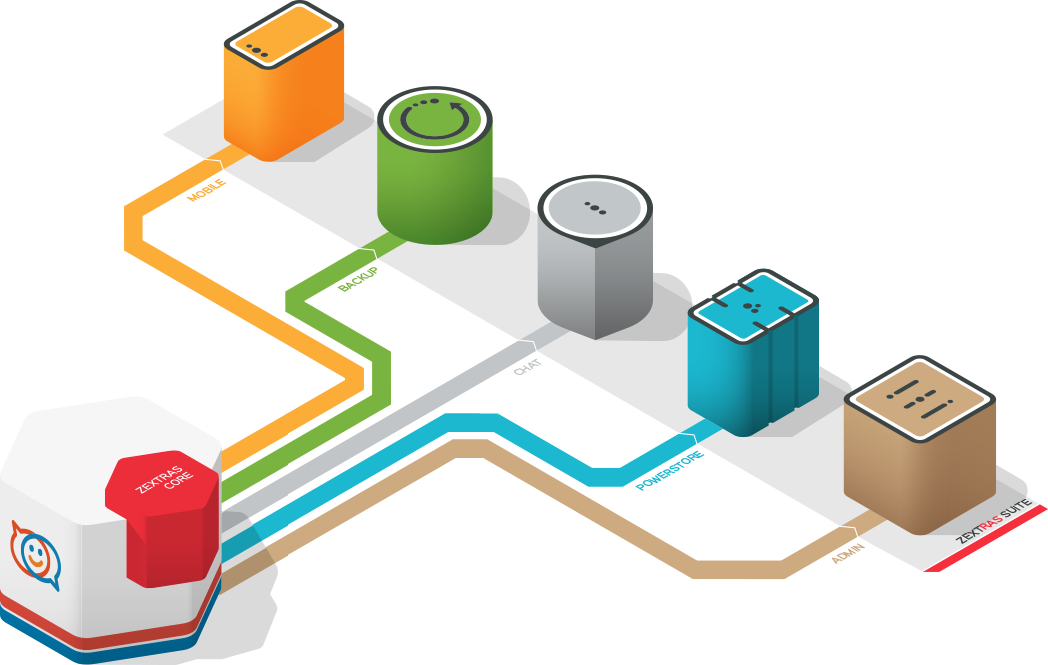
\includegraphics[width=0.7\textwidth]{immagini/zextras_suite.png}
            \caption{Zextras \textit{suite}}
            \textbf{Fonte}: \href{https://www.zimbra-zextras.pl/}{zimbra-zextras.pl}
            \label{fig: Zextras suite}
        \end{figure}
        
\section{Struttura interna}
    L'azienda è suddivisa in diversi settori specializzati, ciò permette di avere un organico fornito di tutte le competenze necessarie per raggiungere gli obiettivi prefissati. Di seguito un elenco che illustra i diversi reparti:
    \begin{itemize}
        \item \textbf{Commercio}: questo reparto, facente parte di \textbf{Studio Storti}, si occupa di gestire tutto ciò che riguarda la parte commerciale e \textit{marketing} dei prodotti proposti dall'azienda;
        \item \textit{\textbf{System administration}}: questo \textit{team} svolge l'attività di gestione e manutenzione dell'infrastruttura interna all'azienda che ospita numerosi \textit{server}, i quali erogano i servizi offerti da \gls{zcsg} ai clienti;
        \item \textbf{\textit{Team} di sviluppo}:
            il \textit{team} di sviluppo è suddiviso in più aree, ognuna delle quali lavora su un aspetto specifico dei prodotti di \textbf{Zextras}:
            \begin{itemize}
                \item \textit{\textbf{Front-end}}: questa divisione progetta e sviluppa tutto ciò che riguarda l'interfaccia grafica delle applicazioni \textit{web};
                \item \textit{\textbf{Back-end}}: questo \textit{team} si occupa di progettare e implementare l'architettura di tutti i servizi offerti dai prodotti dell'azienda. \'E ulteriormente suddiviso in due \textit{team}, ciascuno responsabile di un insieme di prodotti diverso;
                \item \textit{\textbf{UI/UX Design}}: si occupa di progettare l'interfaccia grafica e di studiare l'\textit{\gls{userexpg}} delle applicazioni \textit{web}. Lavora a stretto contatto con la divisione \textit{front-end};
                \item \textit{\textbf{Mobile}}: progettazione e sviluppo delle applicazioni per dispositivi mobili.
            \end{itemize}
    \end{itemize}

\newpage

\section{Processi aziendali}
    I processi sono un tassello di estrema importanza all'interno di un'azienda che si pone degli obiettivi ben definiti, soprattutto quando questi sono particolarmente ambiziosi e raggiungibili tramite lo sviluppo di prodotti complessi e di grandi dimensioni. Sono inoltre fondamentali qual\'{o}ra l'azienda avesse al suo interno dei reparti che svolgono mansioni molto differenti tra loro. \\
    Per orchestrare e mettere in funzione tutti i settori dell'azienda affinché questi lavorino in modo coeso, è necessario ricorrere alla definizione e istanziazione di processi, i quali permettono di stabilire con precisione quali sono le attività da svolgere e il modo più strategico per portarle a termine, al fine di raggiungere gli obiettivi prefissati.
    
    \begin{figure}[ht]
        \centering
        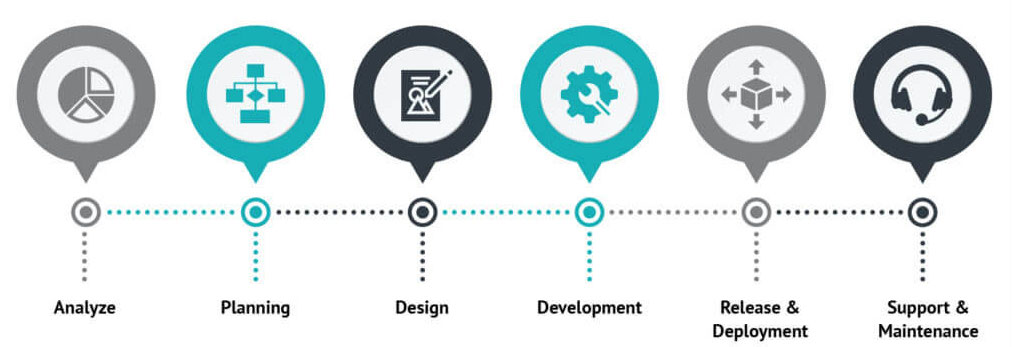
\includegraphics[width=1\textwidth]{immagini/process.jpg}
        \caption{Processi}
        \textbf{Fonte}: \href{https://www.keyideasinfotech.com/wp-content/uploads/blog/Web-and-e-commerce-software-development-processes.jpg}{keyideasinfotech.com}
        \label{fig: Processi}
    \end{figure}
    
    \subsection{Fornitura}
        La grande diffusione di \gls{zcsg} in molteplici ambiti, contribuisce alla necessità di nuove funzionalità e al miglioramento di quelle già esistenti. Per questo motivo \textbf{Zextras} ottiene spesso nuovi incarichi e nuovi progetti da sviluppare. \\
        La ricerca di nuovi progetti avviene tramite il \textit{CEO} dell'azienda e il \textit{Project Manager}. Oltre all'esigenze dei clienti, nascono dei progetti anche interni all'azienda stessa derivanti, ad esempio, dalla necessità di migliorare i processi interni con dei nuovi strumenti. \\
        Una volta individuato un possibile progetto, viene fissata una riunione alla quale partecipano i responsabili e il \textit{team} di sviluppo (formato da gruppi appartenenti a più reparti) che dovrà poi occuparsi del ciclo di vita del nuovo prodotto. Per progetti di grandi dimensioni o particolarmente complessi, la fase di studio di fattibilità dura più tempo e prevede un numero maggiore di riunioni, durante le quali si cerca fin da subito di individuare possibili soluzioni ad alto livello per valutarne la fattibilità. \\
        Dalle riunioni effettuate vengono generati dei verbali, dai quali si estraggono le informazioni più rilevanti che andranno a contribure ai primi contenuti della documentazione. \\
        Quando la soluzione viene approvata da azienda e cliente, si procede con le fasi successive.
    \subsection{Comunicazione}
        Una comunicazione efficiente all'interno del nucleo aziendale è fondamentale per poter essere tutti allineati e coordinati, soprattutto quando è necessario interagire con membri di altri \textit{team} collocati in altre aree dell'azienda.
        \subsubsection{Strumenti utilizzati}
        \begin{itemize}
            \item \textbf{Posta elettronica}: servizio offerto tramite la posta elettronica di \gls{zcsg};
            \item \textit{\textbf{Team}}: piattaforma di messaggistica istantanea integrata in \gls{zcsg} sviluppata da \textbf{Zextras};
            \item \textit{\textbf{Drive}}: piattaforma per la condivisione di documenti su \textit{server} sviluppata dall'azienda;
            \item \textbf{Riunioni}: per discussioni con tutti i membri (o una parte) del \textit{team}, è possibile indire delle brevi riunioni.
        \end{itemize}

\subsection{Metodologia di sviluppo}\label{sec:met_svilpuppo}
    Per sostenere lo sviluppo di software complessi e dalle dimensioni sostanziose, è necessario avere a disposizione una certa flessibilità ed essere pronti a possibili cambiamenti in termini di requisiti, data anche la tiplogia di servizi che l'azienda offre. Per questo motivo \textbf{Zextras} adotta una filosofia \textit{\gls{agileg}}, preferita rispetto a modelli più rigorosi con l'istanziazione di processi molto forti che portano ad una minore capacità di reagire a cambiamenti imminenti. In particolare, la metodologia di sviluppo adottata in azienda è \textit{Scrum}. In seguito descriverò \textit{Scrum} in relazione a come l'azienda lo attua e a quello che concerne la mia esperienza di stage. \\
    Lo sviluppo di un progetto viene suddiviso in fasi, chiamati \textit{Sprint}, la cui durata può variare da una a quattro settimane. In questo caso, la durata dello \textit{Sprint} era di due settimane.
    Ciascuno \textit{Sprint} ha uno o più obiettivi da portare a termine entro la fine di esso.
    Il \textit{\gls{frameworkg}} \textit{Scrum} prevede lo svolgimento di alcuni eventi e di seguito saranno descritti quelli effettivamente svolti:
    
    \begin{itemize}
        \item \textit{\textbf{Sprint Planning}}: si tratta di una riunione che viene indetta all'inizio di ogni \textit{Sprint}, durante la quale vegono discussi gli obiettivi da raggiungere (\textit{Sprint Goal}). Nello specifico, lo \textit{Scrum Master} ovvero colui che coordina il team sceglie, insieme ai colleghi, i \textit{\gls{taskg}} da svolgere nel corso dello \textit{Sprint} e li inserisce nello \textit{Sprint Backlog}. I \textit{\gls{taskg}} vengono scelti dal \textit{Product Backlog}, ovvero dalla lista completa di funzionalità da implementare nel prodotto. Vengono inoltre stabilite le ore che ciascun membro del \textit{team} potrà e dovrà dedicare allo sviluppo, alle riunioni e ad altre attività durante il prossimo \textit{Sprint};
        \item \textit{\textbf{Daily Scrum}}: è una riunione della durata di circa 15 minuti che viene svolta ogni inizio giornata con il \textit{team} di sviluppo (ed eventuali altre persone coinvolte) chiamato anche \textit{Stand-up meeting}. Duranta questa riunione ciascun membro del \textit{team} parla di ciò che ha svolto il giorno precedente, se ha incontrato ostacoli nello svolgere i suoi \textit{\gls{taskg}} e su quali lavorerà durante la giornata. Per più della metà dello stage, i \textit{daily scrum} del mio \textit{team} si sono svolti in lingua inglese al fine di migliorare le abilità linguistiche;
        \item \textit{\textbf{Sprint Retrospective}}: questo evento prevede una riunione in cui il \textit{team} esegue una valutazione retrospettiva sull'andamento dello \textit{Sprint} appena concluso. In particolare vengono analizzate le metriche riguardanti il numero di \textit{\gls{taskg}} portati a termine e gli obiettivi raggiunti. Durante questa riunione viene inoltre svolta un'altra importante attività, ovvero la discussione delle abitudini del \textit{team} e la ricerca di nuove \textit{best practice}. Per fare ciò, ricorre allo \textit{Starfish Retrospective}, uno schema in cui è possibile individuare i seguenti punti:
            \begin{itemize}
                \item \textit{\textbf{More of}}: elenco delle attività che svolte con più frequenza gioverebbero alla crescrita del \textit{team} e allo sviluppo del prodotto;
                \item \textit{\textbf{Less of}}: elenco delle attività da ridurre;
                \item \textit{\textbf{Start doing}}: nuove attività individuate di recente che potrebbero migliorare il \textit{team} e il prodotto;
                \item \textit{\textbf{Keep doing}}: attività che è utile continuare a svolgere;
                \item \textit{\textbf{Stop doing}}: attività il cui svolgimento va interrotto poiché non più necessario oppure perché si tratta di una \textit{bad practice}.
            \end{itemize}
            
            \begin{figure}[h]
                \centering
                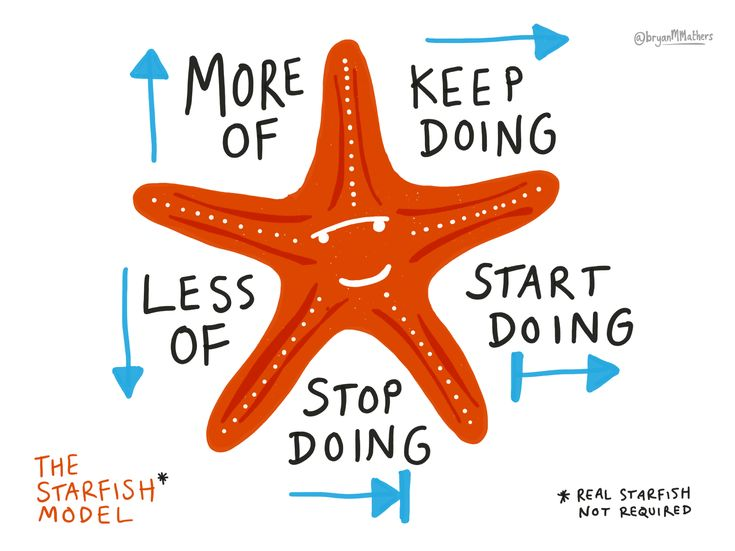
\includegraphics[width=0.7\textwidth]{immagini/starfish.jpg}
                \caption{\textit{Starfish retrospective}}
                \textbf{Fonte: }\href{https://bryanmmathers.com/the-starfish-model/}{bryanmathers.com}
                \label{fig: Starfish retrospective}
            \end{figure}
            
        \item \textit{\textbf{Backlog Refinement}}: questa attività, svolta durante lo \textit{Sprint Planning}, consiste nel controllare che tutti gli \textit{item} presenti nel \textit{Product Backlog} siano pronti per essere selezionati e inseriti nello \textit{Sprint Backlog}. Ne vengono rivisti i contenuti, le priorità, le persone assegnate per il loro svolgimento e, se necessario, vengono suddivisi in \textit{\gls{taskg}} più piccoli o inclusi in altri già esistenti.
    \end{itemize}
    
    \begin{figure}[ht]
        \centering
        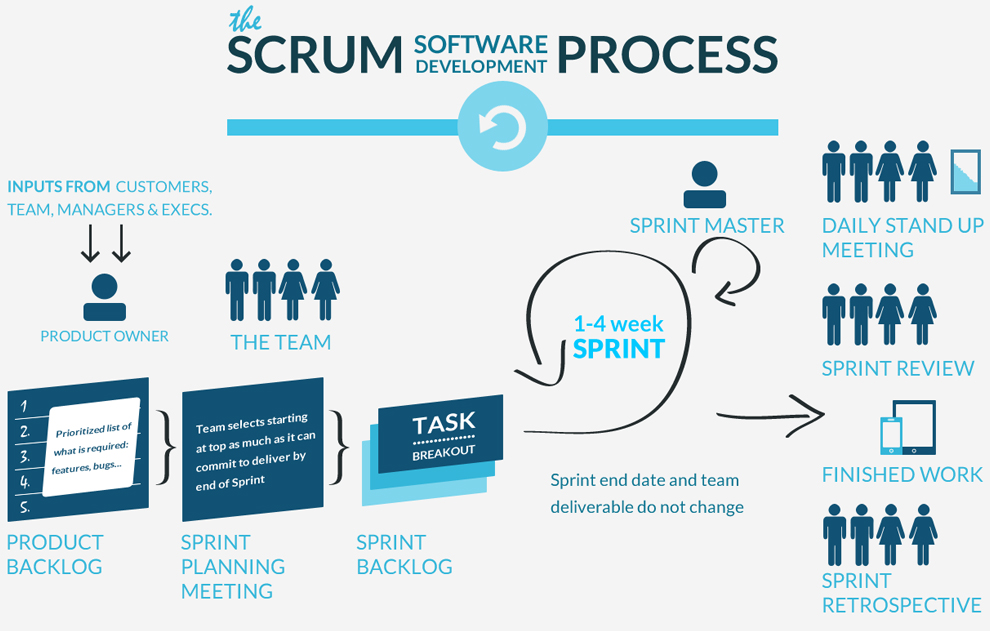
\includegraphics[width=1\textwidth]{immagini/scrum.jpg}
        \caption{Scrum \textit{flow}}
        \textbf{Fonte:} \href{https://www.ics.ie/news/view/1653}{ICS}
        \label{fig: Scrum flow}
    \end{figure}

\newpage

\subsection{Gestione di progetto}
    La gestione del progetto viene supportata principalmente da due strumenti:
    \begin{itemize}
        \item \textbf{Atlassian Jira}: è un \textit{\gls{itsg}} molto avanzato che offre la possibilità di gestire tutto ciò che riguarda il \textit{\gls{frameworkg}} \textit{Scrum}, quindi gestione degli \textit{Sprint}, dei \textit{\gls{taskg}} e molto altro. Da \textbf{Jira} è inoltre possibile tracciare le ore impiegate per portare a termine ciascun \textit{\gls{taskg}} fornendo, al termine dello \textit{Sprint}, delle serie storiche con i tempi impiegati dai membri del \textit{team} e il numero di \textit{\gls{taskg}} portati a termine rispetto a quelli previsti nello \textit{Sprint Backlog}; 
        \item \textbf{\gls{zcsg}}: offre, tra i tanti servizi, il calendario per la gestione degli eventi interni all'azienda, per esempio le riunioni e la possibilità di lavorare su documenti condivisi, per esempio i fogli di calcolo utilizzati per il tracciamento delle ore durante lo \textit{Sprint Planning} come descritto nella sezione \secref{sec:met_svilpuppo}. 
    \end{itemize}

\subsection{Documentazione}\label{sec:doc}
    La documentazione di tutti i \textit{team} di sviluppo è raccolta in un unico punto accessibile a tutti. Per ottenere ciò viene utilizzato il \textit{software} di collaborazione \textbf{Confluence} sviluppato da \textbf{Atlassian}, il quale offre un \textit{editor} di tipo \textit{\gls{wysiwygg}} che permette di scrivere documenti completi e ben formattati oltre a fornire un sistema di catalogazione molto flessibile e personalizzabile.

\newpage

\subsection{Configurazione}\label{sec:configurazione}
Gli strumenti per il versionamento del codice utilizzati sono i seguenti:
\begin{itemize}
    \item \textbf{Git}: sistema di versionamento;
    \item \textbf{Bitbucket}: servizio che ospita i \textit{\gls{repositoryg}} di tutti i \textit{team} di sviluppo. Il vantaggio di usare questo strumento è la sua completa integrazione con tutti gli altri strumenti di \textbf{Atlassian} impiegati dall'azienda;
    \item \textbf{GitHub}: servizio che ospita i \textit{\gls{repositoryg}} \textit{\gls{opensg}} dell'azienda.
\end{itemize}
Per lo sviluppo di nuove funzionalità viene utilizzato un \textit{\gls{workflowg}} molto simile a \textbf{Gitflow}\footnote{\url{https://danielkummer.github.io/git-flow-cheatsheet/}}. Il funzionamento è il seguente:
\begin{enumerate}
    \item Creazione di un nuovo \textit{branch} sul quale sviluppare una nuova funzionalità;
    \item Implementazione della nuova funzionalità;
    \item \textit{Pull request} per effettuare il \textit{merge} del codice sul \textit{branch master}, nella quale vengono inseriti alcuni membri del \textit{team} come revisori che effettueranno una \textit{\gls{codereviewg}}, la quale permette di verificare che il codice sia in linea con gli standard di qualità.
    \item Dopo aver messo a punto le correzioni segnalate nella \textit{\gls{codereviewg}} e aver ricevuto l'approvazione dai revisori, avviene il \textit{merge} sul \textit{branch master}.
\end{enumerate}
    \begin{figure}[ht]
        \centering
        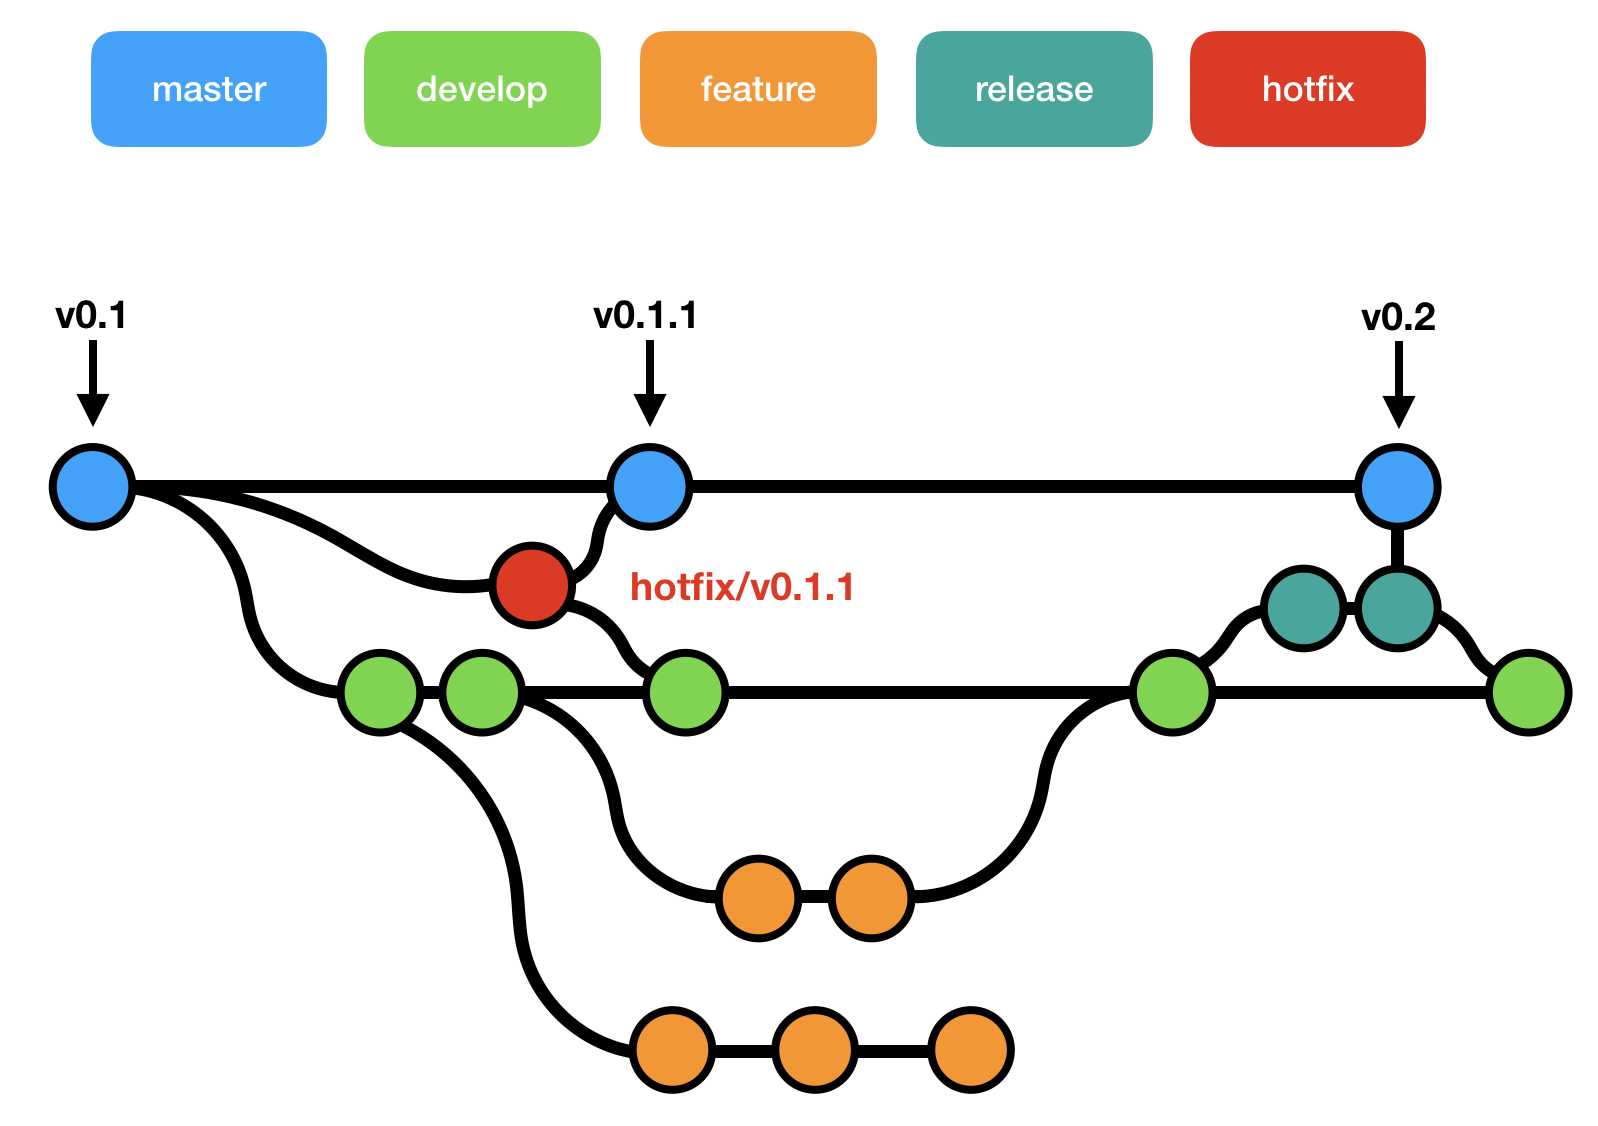
\includegraphics[width=0.8\textwidth]{immagini/git_flow.png}
        \caption{\textit{Gitflow}}
        \textbf{Fonte:} \href{https://www.codewall.co.uk/a-git-flow-explainer-how-to-tutorial/}{codewall.co.uk}
        \label{fig: Gitflow}
    \end{figure}

\newpage

\subsection{Verifica}\label{sec:verifica}
    La verifiche che permettono di perseguire la qualità di prodotto avvengono tramite \textbf{Jenkins}, un \textit{automation server} che supporta la \textit{\gls{cig}} e la \textit{\gls{cdg}}.
    In questo modo è possibile automatizzare il processo di \textit{build} ed esecuzione delle varie tipologie di \textit{test} ad ogni \textit{commit} sul \textit{\gls{repositoryg}} e rilasciare quest'ultima in ambiente di produzione.
    \textbf{Jenkins} permette di aggiungere altre funzionalità al processo di \textit{build}, per esempio l'analisi statica del codice, la rilevazione di alcune tipologie di \textit{\gls{bugg}} e il \textit{code coverage}, rendendolo quindi uno strumento molto flessibile e personalizzabile.
    Prima della verifica automatizzata vengono effettuate le \textit{\gls{codereviewg}} come descritto nella sezione precedente.
    

    \begin{figure}[ht]
        \centering
        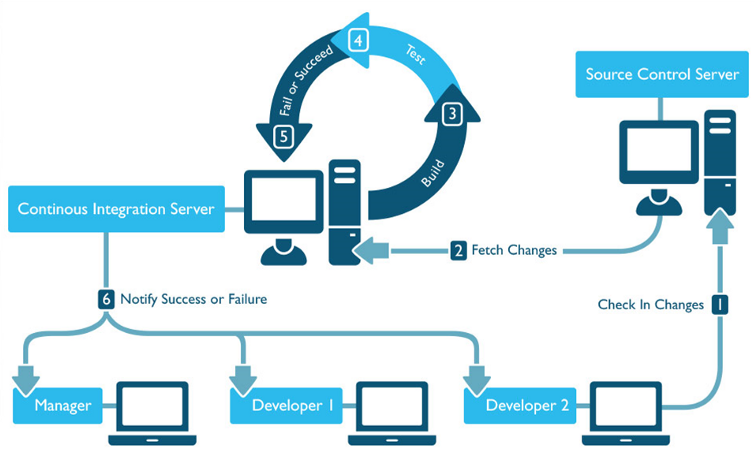
\includegraphics[width=1\textwidth]{immagini/ci.png}
        \caption{\textit{Continuous Integration}}
        \textbf{Fonte:} \href{https://developers.redhat.com/blog/2017/09/06/continuous-integration-a-typical-process/}{developers.redhat.com}
        \label{fig: Continuous Integration}
    \end{figure}
             % Introduzione
% !TEX encoding = UTF-8
% !TEX TS-program = pdflatex
% !TEX root = ../tesi.tex

%**************************************************************
\chapter{Obiettivi dello stage}
\label{cap:obiettivi}
%**************************************************************

% SSO IMAGE SOURCE https://www.getkisi.com/courses/sso-guide

\section{Presentazione del progetto}
    Questo progetto nasce dall'esigenza di avere un sistema di autenticazione per la \textit{webmail} di \gls{zcsg} che fornisse il giusto connubio tra sicurezza e facilità d'uso. \textbf{Zextras} utilizza molti strumenti e servizi al suo interno, sia per lo sviluppo sia per l'amministrazione. Tutti questi servizi utilizzano \gls{okta} per la gestione dell'autenticazione, ciò significa che è sufficiente effettuare una sola autenticazione con il proprio account su \gls{okta} per poter poi accedere a tutti i servizi ad esso collegati. \\
    Questa tipologia di autenticazione si chiama \gls{sso} e consiste nell'utilizzo di una singola credenziale che permette di accedere a più servizi diversi. \\
    \gls{zcsg} era l'unico serivizio, uno dei più estensivamente utilizzati in azienda, che non beneficiava di questa tecnica di autenticazione. Per questo motivo \textbf{Zextras} prende la decisione di esplorare la possibilità di svilupparne una personalizzata che, oltre all'autenticazione base, avesse le seguenti caratteristiche:
    \begin{itemize}
        %\setlength\itemsep{0em}
        \item quando un utente che possiede un \textit{account} su \gls{okta} ma non su \gls{zcsg}, accede per la prima volta su quest'ultima, viene creato un nuovo account su \gls{zcsg}, associato a quello di \gls{okta};
        \item importazione su \gls{zcsg} delle informazioni utente presenti su \gls{okta};
        \item sincronizzazione dei gruppi di \gls{okta} ai quali un utente appartiene, con liste di distribuzione e classi di servizio di \gls{zcsg}.
    \end{itemize}
    Il fine di questo progetto era quello di uniformare il metodo di autenticazione di \gls{zcsg} rispetto a tutti gli servizi utilizzati dall'azienda e soprattutto avere un sistema personalizzato e configurabile che permette di automatizzare alcune operazioni ripetitive e dispendiose in termini di tempo.
    Per poter proporre una soluzione conforme alle esigenze emerse, ho dovuto per prima cosa condurre uno studio e un'analisi dei protocolli di autenticazione presenti sul mercato. La seconda parte invece consisteva nella progettazione e implementazione del sistema utilizzando il protocollo più idoneo.
    
    \begin{figure}[h]
        \centering
        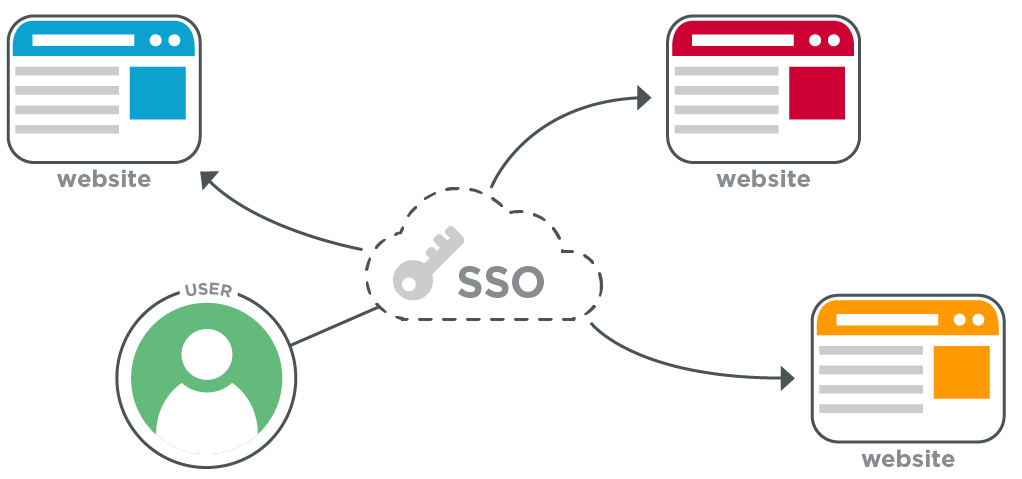
\includegraphics[width=0.75\textwidth]{immagini/sso.png}
        \caption{Single Sign-On}
        \textbf{Fonte}:
        \href{https://developer.fourth.com/en-gb/docs/single-sign-saml}{developer.fourth.com}
        \label{fig: Single Sign-On}
    \end{figure}

\newpage

    \subsection{Analisi stato dell'arte protocolli di autenticazione}\label{sec:att_analisi}
    %Descrizione dell'attività di analisi e di studio dei protocolli di autenticazione che ho dovuto condurre come prima attività durante lo stage.
    La prima attività che ho dovuto svolgere era la ricerca e lo studio dei protocolli di autenticazione più diffusi e utilizzati sul mercato. L'azienda conosceva già alcuni di questi, ma voleva avere un'analisi approfondita e degli scenari pratici. Inoltre poteva rivelarsi una valida occasione per scoprire nuovi possibili protocolli adatti all'implementazione del sistema di autenticazione. \\
    L'azienda ha quindi richiesto di redigere un documento che riportasse tutti i risultati delle mie ricerche, in particolare l'analisi dei pro e dei contro di ciascun protocollo e se questo potesse essere idoneo al nostro caso d'uso.

    \subsection{Progettazione di un sistema di autenticazione personalizzato}
        In seguito all'analisi svolta, il secondo obiettivo dello stage era la progettazione, seguita dall'implementazione, di un sistema di autenticazione per \gls{zcsg} utilizzando il protocollo ritenuto più idoneo. Il sistema di autenticazione doveva essere in grado di:
        \begin{itemize}
            \setlength\itemsep{0em}
            \item utilizzare \gls{okta} come \gls{idpg};
            \item supportare altri \gls{idpg} che utilizzato lo stesso protocollo;
            \item supportare \gls{zcsg} tramite il \gls{ssog} di \gls{okta} rendendo opzionale l'accesso tramite \textit{email} e \textit{password};
            \item garantire sicurezza.
        \end{itemize}
    \newpage
    \begin{figure}[h]
        %\setlength{\textfloatsep}{1pt}
        %\setlength{\belowcaptionskip}{1pt}
        \centering
        
\includegraphics[width=0.75\textwidth]{immagini/rd.jpg}
        \caption{\textit{Research \& Development}}
        \textbf{Fonte}:
        \href{https://youteam.io/blog/research-and-development-the-fourth-pillar-of-software-development/}{youteam.io}
        \label{fig: Research & Development}
    \end{figure}
    
\section{Vantaggi aziendali}
    \textbf{Zextras} ospita stage di questa tipologia da ormai diversi anni nonostante sia un'attività che richiede un quantità di tempo e impegno non indifferente poiché è costretta a sottrarre risorse dai progetti e dalle attività in corso che, molto spesso, sono vincolate da scadenze. Tuttavia i vantaggi portati da uno strumento come lo stage sono molteplici. Per prima cosa l'azienda ha la possibilità di condurre dei progetti di ricerca che molto spesso coinvolgono l'utilizzo di nuove tecnologie, senza essere costretta a rallentare lo sviluppo dei prodotti ordinari e soprattutto riducendo il rischio di investire troppe risorse in progetti che potenzialmente potrebbero non proseguire. \\
    Un altro aspetto interessante dal punto di vista aziendale è il poter entrare in contatto con studenti che, seppur privi di esperienza lavorativa, sono spesso in grado di proporre soluzioni alternative e creative a problemi comuni. I vantaggi elencati si sono effettivamente concretizzati nel tempo, infatti negli utlimi anni il team di sviluppo ha integrato nel suo organico alcuni studenti che, una volta completato lo stage, sono rimasti a contribuire alle sfide tecnologiche che l'azienda affronta giornalmente. \\
    %Alcuni progetti di stage proposti sono molto strategici e hanno altri obiettivi oltre al progetto in sè. Per esempio, l'azienda può sfruttare questo strumento per poter inserire un nuovo 
    Ciò significa che uno stage ben organizzato e seguito si rivela essere un vero e proprio investimento, non solo per l'azienda che lo ospita, la quale beneficerà degli \textit{output} di questo strumento, ma anche per la crescita degli studenti, i quali saranno le figure professionali che nel futuro faranno parte dell'intera industria che al giorno d'oggi necessita di molte risorse vista la sua dinamicità.

\newpage

\section{Vincoli}
    \subsection{Vincoli metodologici}
        Per lo svolgimento dell'attività di stage è stato deciso, in comune accordo con il \textit{tutor}, che il modo più efficace per portarla a termine fosse lavorare presso la sede aziendale. La prima motivazione deriva dalla metodologia di sviluppo adottata, descritta nella sezione \secref{sec:met_svilpuppo}, la quale è fortemente incentrata sulla comunicazione e sul confronto con tutti i membri nel \textit{team}. Inoltre, poiché sarei stato affiancato da alcuni \textit{senior developer} si trattava di un'ottima occasione per apprendere il più possibile da professionisti nel settore. \\
        Oltre agli incontri di allineamento giornalieri, il \textit{Project Manager} ha stabilito che ci sarebbero stati degli incontri formali, insieme al \textit{tutor} aziendale, per fare il punto della situazione. Nella fase conclusiva del progetto era inoltre prevista una \textit{\gls{demog}} a cui avrebbero presenziato:
        \begin{itemize}
            \item il \textit{CEO} dell'azienda;
            \item il \textit{Project Manager};
            \item il responsabile tecnico dell'azienda;
            \item il \textit{team} di sviluppo con il \textit{tutor} aziendale;
            \item il responsabile di un altro \textit{team};
        \end{itemize}
        La presenza di figure appartenti a diversi settori e \textit{team} sarebbe state utile a discutere il prodotto sviluppato, sia dal punto di vista funzionale sia da quello infrastrutturale. Inoltre, ricevere un \textit{feedback} da punti di vista diversi è certamente utile per il miglioramento dell'applicazione nel suo insieme.
        
        \begin{figure}[h]
            \centering
            
\includegraphics[width=0.8\textwidth]{immagini/team.jpg}
            \caption{\textit{Teamwork}}
            \textbf{Fonte}:
            \href{https://www.sandler.com/blog/6-benefits-of-teamwork-in-the-workplace/}{sandler.com}
            \label{fig: Teamwork}
        \end{figure}
        
    \subsection{Vincoli temporali}
    L'attività di stage prevista aveva una durata di 304 ore, da svolgere nell'arco di due mesi, suddivise in 8 settimane della durata di circa 40 ore ciascuna. L'orario di lavoro accordato con l'azienda era dal Lunedì al Venerdì dalle ore 9.00 alle 18.00. \\
    Prima dell'inizio dello stage ho pianificato, insieme al \textit{tutor} le attività per ciascuna settimana di lavoro, facendone una stima orario per il completamento. Sin dal primo giorno io e il \textit{tutor} aziendale abbiamo rispettato il piano di lavoro stabilito. Tuttavia, in seguito all'attività di analisi svolta, come descritto nella sezione \secref{sec:att_analisi}, abbiamo dovuto dedicare più tempo per ottenere un prototipo base funzionante, poiché non era ancora chiaro come utilizzare il protocollo di autenticazione scelto. Nonostante un rallentamento a metà percorso, il resto dello stage ha avuto un andamento lineare che mi ha permesso di terminare il lavoro senza fretta. 
    
    \begin{figure}[h]
        \centering
        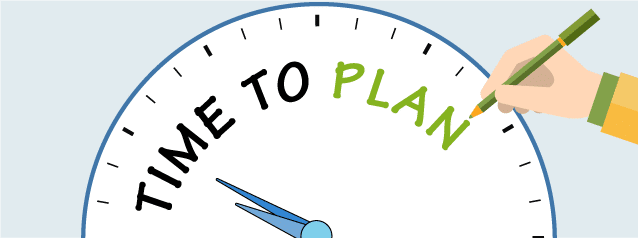
\includegraphics[width=1\textwidth]{immagini/plan.png}
        \caption{\textit{Planning}}
        \textbf{Fonte}:
        \href{https://www.sysaid.com/blog/entry/8-tips-on-how-to-plan-for-configuration-management-part-1}{sysaid.com}
        \label{fig: Planning}
    \end{figure}
    
    \subsection{Vincoli tecnologici}
    Le tecnologie e i linguaggi utilizzati duarante questo progetto dello \textit{stack} tecnologico dell'azienda e sono le seguenti:
    \begin{itemize}
        \item \textbf{Java}: essendo il linguaggio con cui è scritto \gls{zcsg}, ne consegue che tutta la tecnologia di \textbf{Zextras} si sia adeguata, compreso il mio progetto;
        \item \textbf{Git}: sistema di versionamento, come descritto nella sezione \secref{sec:configurazione};
        \item \textbf{Docker}: è una tecnologia che permette di creare, rilasciare ed eseguire delle applicazioni utilizzando i \gls{containerg}. In questo modo il \gls{containerg} potrà essere eseguito, tramite \textit{docker}, su macchine diverse che solitamente sono configurate in diversi modi. Questo comportamente è simile alla virtualizzazione e permette di rendere gli ambienti di esecuzione solidi e deterministici. In particolare l'azienda lo utilizza per creare delle istanze di \gls{zcsg} utilizzate come ambienti di test in fase di sviluppo. In azienda i \gls{containerg} di \textit{docker} sono gestiti tramite un servizio di nome \textbf{\textit{Portainer}}\footnote{https://www.portainer.io/}.
    \end{itemize}

\section{Aspettative aziendali}
%Descrizione degli output che l'azienda si aspettava da questo stage
Al termine delle 304 ore previste per il completamento dello stage, l'azienda si aspettava di avere almeno un prototipo funzionante che facesse uso di un protocollo di autenticazione, al fine di permettere l'autenticazione su \gls{zcsg} tramite l'\gls{idpg} \gls{okta}. Come già descritto in precedenza però, la parte interessante di questo progetto era l'aggiunta di alcune funzionalità personalizzate ad un sistema di autenticazione standard. Per questo motivo dopo aver concluso l'attività di ricerca sui protocolli, descritta nel paragrafo \secref{sec:att_analisi}, ho discusso, insieme al \textit{team} e al \textit{Project Manager}, i requsiti specifici da implementare. Ciò è stato utile perché al momento della stesura del piano di lavoro, alcuni di essi non potevano essere a me chiari, causa mancanza di contesto riguardante l'ambiente \gls{zcsg}. Gli obiettivi stabiliti erano suddivisi, in ordine di importanza, in \textbf{obbligatori} e \textbf{desiderabili}.
\paragraph{Obiettivi obbligatori}
\begin{itemize}
    \item Analisi stato dell'arte dei protocolli di autenticazione più diffusi;
    \item Implemenazione di un sistema di autenticazione per \gls{zcsg} tramite il protocollo scelto;
\end{itemize}
\paragraph{Obiettivi desiderabili}
\begin{itemize}
    \item \textit{\gls{prov}};
    \item Importazione dei dati dell'utente da \gls{okta} a \gls{zcsg};
    \item Flusso di autenticazione a partire sia dall'\gls{idpg} sia da \gls{zcsg};
    \item Controllo delle classi di servizio di \gls{zcsg} tramite l'\gls{idpg};
    \item Gestione delle liste di distribuzione di \gls{zcsg} tramite l'\gls{idpg};
    \item Autenticazione a due fattori;
    \item Integrazione con \textit{WebAuthn}\footnote{https://www.w3.org/TR/webauthn-2/}
\end{itemize}

\section{Aspettative personali}
Descrizione di ciò che io mi aspettavo al momento della scelta di questo stage

             % Stage
% !TEX encoding = UTF-8
% !TEX TS-program = pdflatex
% !TEX root = ../tesi.tex

%**************************************************************
\chapter{Resoconto dello stage}
\label{cap:resoconto}
%**************************************************************

\section{Descrizione del progetto}
Descrizione dettagliata del progetto

%**************************************************************
\section{Analisi}
Descrizione dell'analisi dei requisiti e descrizione di alcuni dei requisiti

\section{Pianificazione}
Descrizione di come ho pianificato lo sviluppo del progetto rispettando i vincoli descritti in precedenza e le esigenze dell'azienda

%**************************************************************
\section{Scelta del protocollo di autenticazione}
Descrizione delle motivazioni che hanno portato alla scelta del protocollo SAML in seguito all'analisi svolta
\subsection{Confronto SAML e OpenID}
Breve confronto di due protocolli rispetto al problema da risolvere
\subsection{SAML}
Descrizione del protocollo SAML

\section{Progettazione}
Progettazione della soluzione proposta per l'implementazione del sistema di autenticazione
\subsection{Configurazione applicazione Okta}
\subsection{Progettazione handler HTTP}
\subsection{Configurazione Zimbra}

\section{Sviluppo}
Alcuni dettagli di rilievo per quanto riguarda la parte implementativa. In particolare ciò che ho dovuto attuare per superare alcuni ostacoli
\subsection{Parsing SAML assertion}
\subsection{Adattamento libreria HTTP}

\section{Verifica e Validazione}
Descrizione dell'attività di verifica svolta e della validazione
\subsection{Verifica}
\subsection{Validazione}             % Kick-Off
% !TEX encoding = UTF-8
% !TEX TS-program = pdflatex
% !TEX root = ../tesi.tex

%**************************************************************
\chapter{Valutazione retrospettiva}
\label{cap:retrospettiva}
%**************************************************************

%**************************************************************
\section{Soddisfacimento degli obiettivi}
%Illustrazione degli obiettivi raggiunti rispetto a quelli attesi da me e dall'azienda
Il bilancio degli obiettivi descritti nella sezione \secref{sec:aspettative_aziendali} raggiunti durante lo stage è riassunto nella seguente tabella:

\begin{center}
    \begin{table}[h]
    \def\arraystretch{2}
    \begin{tabular}{|p{9cm}|p{3cm}|} % you can change the dimension according to the spacing requirements 
        \hline
        \textbf{Obiettivo} & \textbf{Stato} \\ \hline  
         Analisi stato dell’arte dei protocolli di autenticazione più diffusi & \textcolor{ForestGreen}{Soddisfatto}\\ \hline
         Implementazione di un sistema di autenticazione per \gls{zcsg} tramite il protocollo scelto & \textcolor{ForestGreen}{Soddisfatto}\\ \hline
         \gls{prov} (creazione dell'\textit{account} su \gls{zcsg})& \textcolor{ForestGreen}{Soddisfatto}\\ \hline
         Importazione dei dati dell’utente di \gls{okta} su \gls{zcsg} & \textcolor{ForestGreen}{Soddisfatto}\\ \hline
         Flusso di autenticazione a partire sia dall’\textit{\gls{idpg}} sia da \gls{zcsg} & \textcolor{ForestGreen}{Soddisfatto}\\ \hline
         Controllo della \gls{cosg} di \gls{zcsg} tramite l’\textit{\gls{idpg}} & \textcolor{ForestGreen}{Soddisfatto}\\ \hline
         Gestione delle \gls{distlistg} di \gls{zcsg} tramite l'\textit{\gls{idpg}} & \textcolor{ForestGreen}{Soddisfatto}\\ \hline
         Autenticazione a due fattori & \textcolor{ForestGreen}{Soddisfatto}\\ \hline
         Integrazione con \textit{WebAuthn}\footnote{\url{https://www.w3.org/TR/webauthn-2/}} & \textcolor{Red}{Non Soddisfatto}\\ \hline
    \end{tabular}
    \caption{Tabella degli obiettivi}
    \end{table}
\end{center}

Come è possibile evincere dalla tabella, ho soddisfatto quasi tutti gli obiettivi prefissati. L'unico obiettivo non soddisfatto è quello relativo all'integrazione con \textit{WebAuthn}\footnote{\url{https://www.w3.org/TR/webauthn-2/}}. Il motivo deriva dal fatto che nella fase avanzata dello sviluppo, l'azienda non era più interessata ad esplorare questa integrazione. Infatti è proprio per questo motivo che ho avuto il tempo di finire tutto il resto del lavoro senza fretta, permettendomi di rilasciare il prodotto e di effettuare le correzioni successive al collaudo. \\
Mi ritengo molto soddisfatto dei risultati ottenuti, perché nella fase iniziale di ricerca non pensavo di andare oltre l'implementazione del sistema di autenticazione base. Questo perché mi aspettavo che l'analisi dei protocolli sarebbe durata più del dovuto, lasciandomi solo il tempo necessario a creare un prototipo. \\
Ho raggiunto l'obiettivo di vivere l'esperienza di lavoro in azienda, nonostante credo che per avere un'idea precisa serva molto più tempo.
Sono riuscito a completare un progetto dall'inizio alla fine, come descritto nella sezione \secref{sec:aspettative_personali}. Partecipare ad un progetto per tutto il suo ciclo di vita e validarlo è, secondo me, un obiettivo importante e soprattutto quantificabile dal punto di vista del bagaglio di esperienza personale.
Il prodotto viene ora utilizzato giornalmente in azienda, ciò significa che ha generato del valore. Questo è particolarmente rilevante per me, poiché l'azienda è anch'essa soddisfatta degli obiettivi raggiunti.

    \begin{figure}[ht]
        \centering
        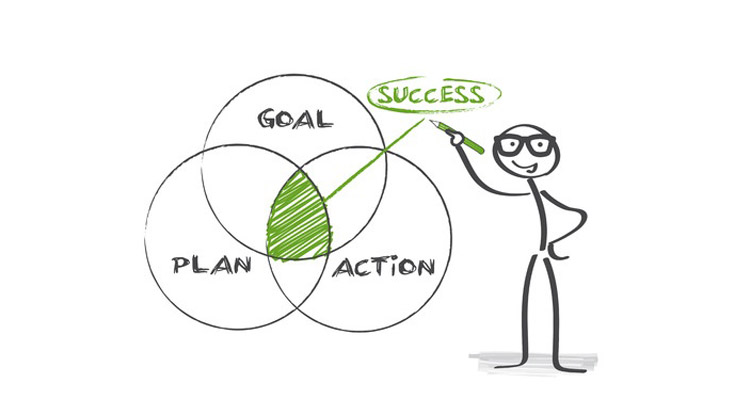
\includegraphics[width=1\textwidth]{immagini/success.jpg}
        \caption{\textit{Goal}}
        \textbf{Fonte}:
        \href{https://brooksplanning.wordpress.com/2016/06/12/action-plan-for-success/
}{brooksplanning.wordpress.com}
        \label{fig: Goal}
    \end{figure}

\newpage

\section{Conoscenze e abilità acquisite}
Questa esperienza si è rivelata molto positiva anche sotto il punto di vista delle conoscenze e competenze che ho acquisito durante i due mesi di stage.
Queste non si limitano solo all'ambito prettamente tecnico ma riguardano anche la realtà aziendale. 
\subsubsection{Azienda}
Ho appreso come un'azienda caratterizza i clienti che utilizzano i suoi prodotti, un aspetto fondamentale dal punto di vista commerciale poiché per creare \textit{software} di successo è necessario che questo abbia dei clienti che lo utilizzino nel tempo. Inoltre ho preso parte ad un contesto aziendale che porta avanti la filosofia del \textit{software} \textit{\gls{opensg}} ed è stato molto interessante vederne le dinamiche. \\
Questo aspetto ha senza dubbio influito sulla scelta del protocollo da utilizzare, in quanto durante lo studio individuale descritto nella sezione \secref{sec:att_analisi}, ho dovuto escludere alcune soluzioni in quanto non compatibili dal punto di vista del tipo di licenza.

\subsubsection{Team di sviluppo}
Ho avuto inoltre modo di lavorare con un \textit{team} di sviluppo completo e di poter collaborare anche con altri reparti dell'azienda che si occupavano di aspetti talvolta distanti dallo sviluppo \textit{software}. Ciò mi ha portato a dover impiegare il giusto linguaggio per comunicare con persone che hanno un punto di vista sul prodotto differente dal mio. \\
Sono rimasto anche sorpreso dal fatto che, nonostante la mia inesperienza, uno dei \textit{senior developer} del \textit{team} mi ha chiesto diverse volte un parere su come avremmo potuto implementare una certa funzionalità. Ciò mi ha fatto comprendere che, nella risoluzione di problemi è molto utile avere diversi pareri pur avendo acquisito un'esperienza considerevole.

\subsubsection{Linguaggi e tecnologie}
Dal punto di vista tecnico ho acquisito alcune conoscenze di cui mi ritengo soddisfatto. Innanzitutto ho potuto osservare e, in parte, mettere in azione in modo professionale alcune tecniche per l'utilizzo di un linguaggio di programmazione (\textit{Java}) da me conosciuto in ambito accademico.
Inoltre ho compreso i vantaggi e le potenzialità di \textit{Docker}, una tecnologia che negli ultimi anni si è ampiamente diffusa sul mercato. \\
Dal punto di vista aziendale mi sono reso conto che le tecnologie vengono sfruttate in tutti i modi possibili per poter raggiungere gli obiettivi. Infatti nel loro impiego può capitare di essere costretti a trovare il giusto compromesso, per esempio tra \textit{performance} e qualità del codice.

\subsubsection{Strumenti}
Ho visto in prima persona come avviene la gestione di un progetto costituito da molte parti e sviluppato da \textit{team} diversi. In particolare l'utilizzo di strumenti di coordinamento come \textbf{Jira} per la gestione di progetto e \textbf{Confluence} per la gestione della documentazione aziendale. \\
Inoltre ho appreso molto dagli sviluppatori \textit{senior} del \textit{team}, i quali mi hanno mostrato come sfruttare al meglio e in modo professionale gli strumenti di sviluppo, al fine di incrementare la produttività e risparmiare tempo.

\subsubsection{Metodo di lavoro}
Oltre ai metodi di lavoro messi in atto dall'azienda, ho potuto sperimentare come condurre la ricerca e lo studio di nuovi argomenti, nel mio caso i protocolli, e come gestire il tempo a disposizione. Tuttavia su questo aspetto ho capito che devo migliorare il mio metodo in quanto, nonostante abbia raggiunto gli obiettivi, non era adeguato per un'analisi approfondita di ciò che stavo studiando. Infatti dopo aver terminato questa attività ho dovuto rivedere alcuni concetti che non avevo ancora compreso completamente.
%**************************************************************
\section{Valutazione personale}
Questa esperienza mi ha fatto riflettere sulla relazione tra il mondo accademico e quello del lavoro. Tutto sommato ritengo che le nozioni apprese durante il corso di laurea triennale siano state molto utili durante questa esperienza, seppur non sufficienti per certi aspetti. \\
Credo che questo meccanismo sia abbastanza naturale poiché l'obiettivo dell'università è quello di erogare conoscenze soprattutto teoriche, necessarie per poter mettere in pratica dei concetti in modo consapevole. Inoltre, essendo il mondo dell'informatica molto ampio, non è pensabile si esplorarlo in soli tre anni. \\
Tuttavia, l'informatica è un campo molto dinamico, cresce e muta anno dopo anno portando alla luce nuovi metodi e tecnologie. Per questo motivo credo che l'offerta didattica erogata dai corsi universitari debba essere adeguatamente aggiornata per poter offrire dei contenuti che siano in linea con ciò che viene utilizzato in ambito professionale. %Inoltre ho notato che molto spesso, quando viene insegnato un linguaggio o una tecnologia, capita che alcune soluzioni vengano etichettate come non ottimali, quando in realtà esistono dei casi d'uso specifici che vengono soddisfatti tramite l'applicazione di tali metodi.
Inoltre avrei preferito che alcuni corsi proponessero degli esempi meno didattici e più concreti, al fine di rendere l'apprendimento più coinvolgente ed efficace. \\
Un modello di insegnamento che ho avuto modo di sperimentare durante questi tre anni, puntava sul fare in modo che lo studente avesse la possibilità di consolidare le conoscenze teoriche con l'ausilio di un progetto didattico significativo, cercando di diminuire il divario tra le conoscenze teoriche e le applicazioni pratiche. In questo caso per esempio, studiare la teoria limitandosi a leggere informazioni presenti nei libri di testo più comuni non era sufficiente, ma era necessario contestualizzarla nell'esperienza vissuta durante il progetto. Nel mio caso, questo metodo è estremamente efficace perché permette di comprendere a fondo i concetti, rendendo quindi poco interessante "ricordare" il loro significato. \\
Nel complesso sono comunque soddisfatto di ciò che mi ha dato l'università, poiché mi ha messo di fronte a nozioni e argomenti che da solo non avrei mai esplorato, anche perché spesso molti aspetti teorici vengono ignorati in campo pratico. In questo modo ho compreso che il modo migliore di risolvere problemi, talvolta complessi, sia quello di unire teoria e pratica in modo strategico. Chiaramente dopo questa esperienza sarò più aperto ad una esplorazione più ampia del mondo dell'informatica, anche dopo aver terminato gli studi. \\
L'attività di stage mi ha pienamente convinto e la consiglio a tutti coloro che hanno la possibilità di farlo, svolto anche in modalità diverse dalla mia, perché è importante per far capire allo studente cosa aspettarsi dal mondo del lavoro e per avere un'idea della tipologia di azienda in cui vuole lavorare.
             % Conclusioni
%\appendix                               
%% !TEX encoding = UTF-8
% !TEX TS-program = pdflatex
% !TEX root = ../tesi.tex

%**************************************************************
\chapter{Appendice A}
%**************************************************************

\epigraph{Citazione}{Autore della citazione}



             % Appendice A

%**************************************************************
% Materiale finale
%**************************************************************
\backmatter
\printglossary[title={Glossario}]
% !TEX encoding = UTF-8
% !TEX TS-program = pdflatex
% !TEX root = ../tesi.tex

%**************************************************************
% Bibliografia
%**************************************************************

\cleardoublepage
\chapter{Bibliografia}

\nocite{*}
% Stampa i riferimenti bibliografici
%\printbibliography[heading=subbibliography,title={Riferimenti bibliografici},type=book]

%Stampa i siti web consultati
\printbibliography[heading=subbibliography,title={Siti web consultati},type=online]


\end{document}
